\documentclass[14pt]{extbook}
\usepackage{multicol, enumerate, enumitem, hyperref, color, soul, setspace, parskip, fancyhdr} %General Packages
\usepackage{amssymb, amsthm, amsmath, bbm, latexsym, units, mathtools} %Math Packages
\everymath{\displaystyle} %All math in Display Style
% Packages with additional options
\usepackage[headsep=0.5cm,headheight=12pt, left=1 in,right= 1 in,top= 1 in,bottom= 1 in]{geometry}
\usepackage[usenames,dvipsnames]{xcolor}
\usepackage{dashrule}  % Package to use the command below to create lines between items
\newcommand{\litem}[1]{\item#1\hspace*{-1cm}\rule{\textwidth}{0.4pt}}
\pagestyle{fancy}
\lhead{Progress Quiz 4}
\chead{}
\rhead{Version C}
\lfoot{4378-7085}
\cfoot{}
\rfoot{Fall 2020}
\begin{document}

\begin{enumerate}
\litem{
Determine the domain of the function below.\[ f(x) = \frac{6}{16x^{2} +32 x + 15} \]\begin{enumerate}[label=\Alph*.]
\item \( \text{All Real numbers except } x = a \text{ and } x = b, \text{ where } a \in [-20.11, -19.61] \text{ and } b \in [-12.18, -11.99] \)
\item \( \text{All Real numbers.} \)
\item \( \text{All Real numbers except } x = a \text{ and } x = b, \text{ where } a \in [-1.45, -0.86] \text{ and } b \in [-0.92, -0.03] \)
\item \( \text{All Real numbers except } x = a, \text{ where } a \in [-20.11, -19.61] \)
\item \( \text{All Real numbers except } x = a, \text{ where } a \in [-1.45, -0.86] \)

\end{enumerate} }
\litem{
Solve the rational equation below. Then, choose the interval(s) that the solution(s) belongs to.\[ \frac{6}{-2x + 5} + -8 = \frac{-8}{-10x + 25} \]\begin{enumerate}[label=\Alph*.]
\item \( x \in [2.02,4.03] \)
\item \( x \in [-3.9,-2.5] \)
\item \( x_1 \in [0.6, 1.7] \text{ and } x_2 \in [2.02,5.03] \)
\item \( x_1 \in [-3.9, -2.5] \text{ and } x_2 \in [2.02,5.03] \)
\item \( \text{All solutions lead to invalid or complex values in the equation.} \)

\end{enumerate} }
\litem{
Solve the rational equation below. Then, choose the interval(s) that the solution(s) belongs to.\[ \frac{7}{-2x + 2} + 4 = \frac{6}{-12x + 12} \]\begin{enumerate}[label=\Alph*.]
\item \( \text{All solutions lead to invalid or complex values in the equation.} \)
\item \( x_1 \in [-0.3, 0.1] \text{ and } x_2 \in [0.75,4.75] \)
\item \( x \in [-0.3,0.1] \)
\item \( x_1 \in [0.6, 1.2] \text{ and } x_2 \in [0.75,4.75] \)
\item \( x \in [0.75,2.75] \)

\end{enumerate} }
\litem{
Choose the graph of the equation below.\[ f(x) = \frac{-1}{x + 2} - 3 \]\begin{enumerate}[label=\Alph*.]
\begin{multicols}{2}\item 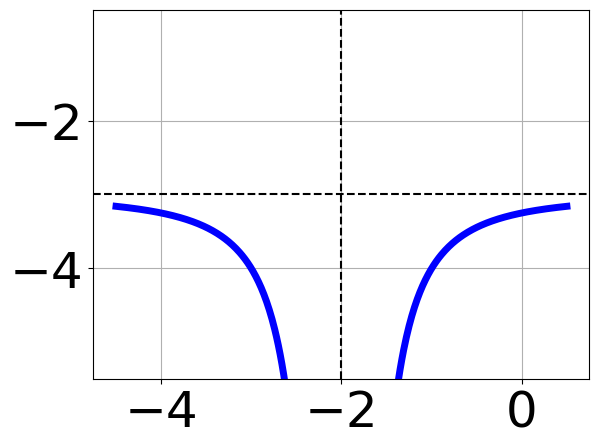
\includegraphics[width = 0.3\textwidth]{../Figures/rationalEquationToGraphAC.png}\item 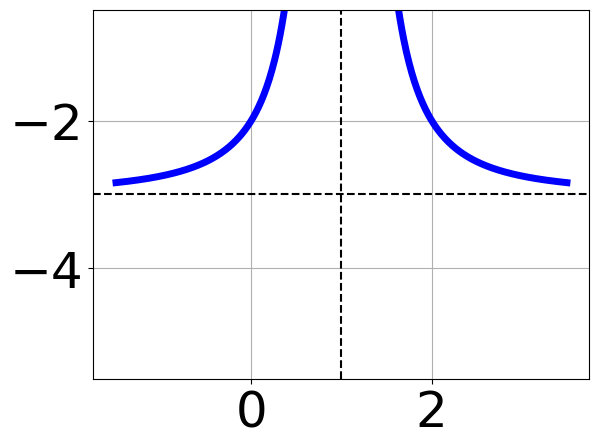
\includegraphics[width = 0.3\textwidth]{../Figures/rationalEquationToGraphBC.png}\item 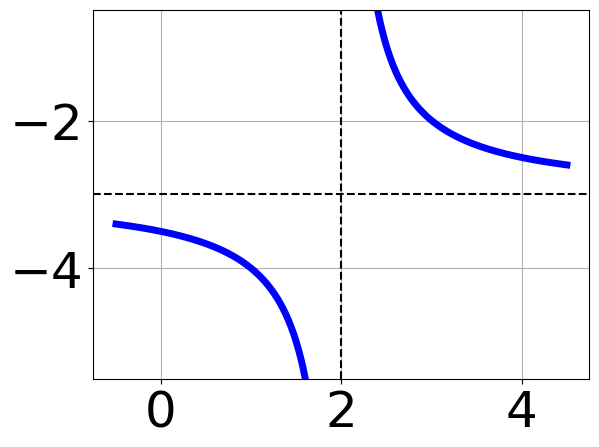
\includegraphics[width = 0.3\textwidth]{../Figures/rationalEquationToGraphCC.png}\item 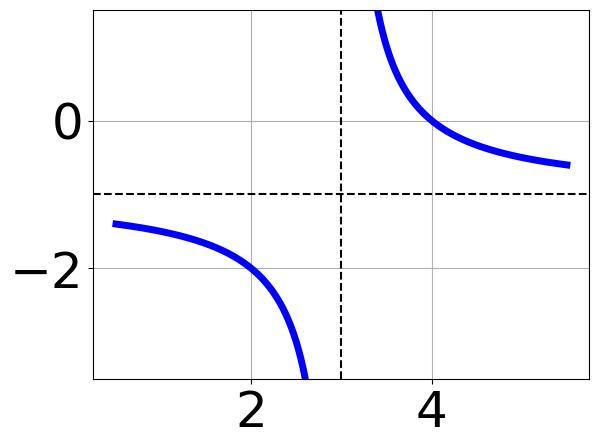
\includegraphics[width = 0.3\textwidth]{../Figures/rationalEquationToGraphDC.png}\end{multicols}\item None of the above.
\end{enumerate} }
\litem{
Determine the domain of the function below.\[ f(x) = \frac{3}{20x^{2} -27 x + 9} \]\begin{enumerate}[label=\Alph*.]
\item \( \text{All Real numbers except } x = a \text{ and } x = b, \text{ where } a \in [11.85, 12.02] \text{ and } b \in [14.48, 15.21] \)
\item \( \text{All Real numbers.} \)
\item \( \text{All Real numbers except } x = a, \text{ where } a \in [11.85, 12.02] \)
\item \( \text{All Real numbers except } x = a, \text{ where } a \in [0.32, 0.71] \)
\item \( \text{All Real numbers except } x = a \text{ and } x = b, \text{ where } a \in [0.32, 0.71] \text{ and } b \in [0.64, 0.85] \)

\end{enumerate} }
\litem{
Choose the equation of the function graphed below.
\begin{center}
    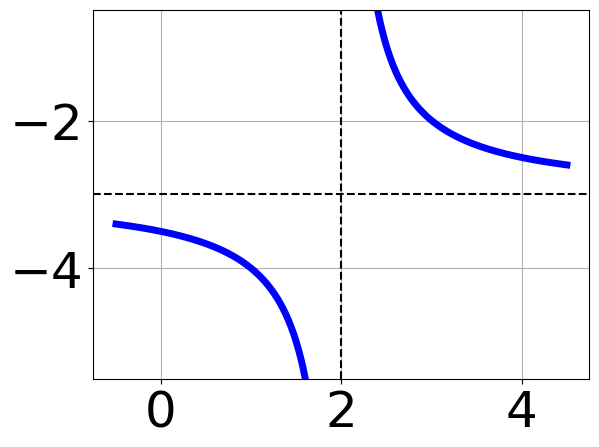
\includegraphics[width=0.5\textwidth]{../Figures/rationalGraphToEquationC.png}
\end{center}
\begin{enumerate}[label=\Alph*.]
\item \( f(x) = \frac{1}{x - 2} - 3 \)
\item \( f(x) = \frac{-1}{x + 2} - 3 \)
\item \( f(x) = \frac{-1}{(x + 2)^2} - 3 \)
\item \( f(x) = \frac{1}{(x - 2)^2} - 3 \)
\item \( \text{None of the above} \)

\end{enumerate} }
\litem{
Solve the rational equation below. Then, choose the interval(s) that the solution(s) belongs to.\[ \frac{-6x}{6x -5} + \frac{-7x^{2}}{-42x^{2} +71 x -30} = \frac{-2}{-7x + 6} \]\begin{enumerate}[label=\Alph*.]
\item \( x_1 \in [-0.32, -0.23] \text{ and } x_2 \in [0.77,0.91] \)
\item \( x \in [0.95,1.01] \)
\item \( x_1 \in [-0.32, -0.23] \text{ and } x_2 \in [0.9,1.05] \)
\item \( \text{All solutions lead to invalid or complex values in the equation.} \)
\item \( x \in [0.77,0.96] \)

\end{enumerate} }
\litem{
Solve the rational equation below. Then, choose the interval(s) that the solution(s) belongs to.\[ \frac{2x}{5x + 7} + \frac{-7x^{2}}{20x^{2} +38 x + 14} = \frac{-6}{4x + 2} \]\begin{enumerate}[label=\Alph*.]
\item \( x_1 \in [-34.16, -32.61] \text{ and } x_2 \in [-1.33,-1.22] \)
\item \( \text{All solutions lead to invalid or complex values in the equation.} \)
\item \( x \in [-2.06,-0.99] \)
\item \( x \in [-0.66,0.49] \)
\item \( x_1 \in [-34.16, -32.61] \text{ and } x_2 \in [-1.55,-1.32] \)

\end{enumerate} }
\litem{
Choose the equation of the function graphed below.
\begin{center}
    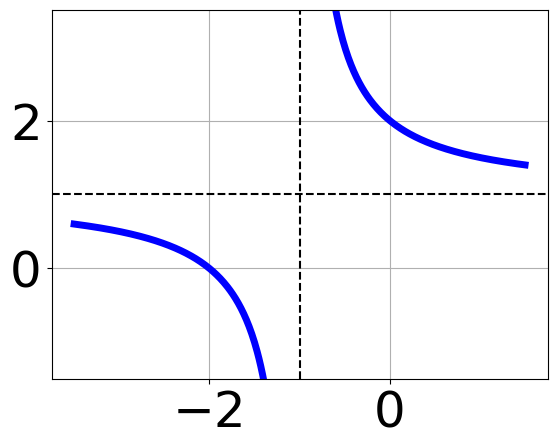
\includegraphics[width=0.5\textwidth]{../Figures/rationalGraphToEquationCopyC.png}
\end{center}
\begin{enumerate}[label=\Alph*.]
\item \( f(x) = \frac{-1}{(x - 2)^2} - 1 \)
\item \( f(x) = \frac{-1}{x - 2} - 1 \)
\item \( f(x) = \frac{1}{x + 2} - 1 \)
\item \( f(x) = \frac{1}{(x + 2)^2} - 1 \)
\item \( \text{None of the above} \)

\end{enumerate} }
\litem{
Choose the graph of the equation below.\[ f(x) = \frac{-1}{x - 2} + 2 \]\begin{enumerate}[label=\Alph*.]
\begin{multicols}{2}\item 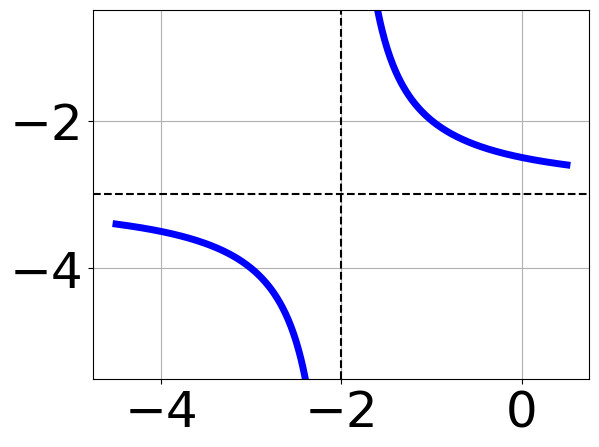
\includegraphics[width = 0.3\textwidth]{../Figures/rationalEquationToGraphCopyAC.png}\item 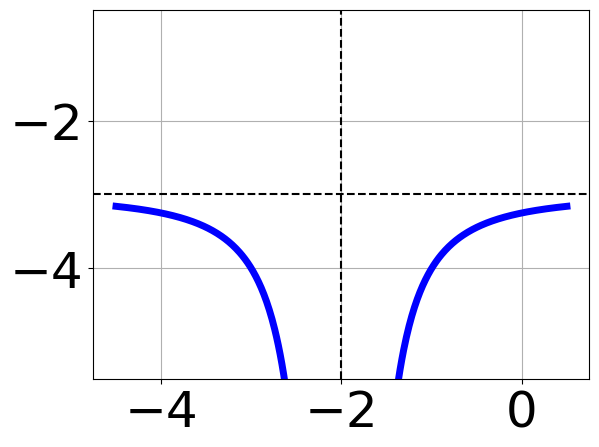
\includegraphics[width = 0.3\textwidth]{../Figures/rationalEquationToGraphCopyBC.png}\item 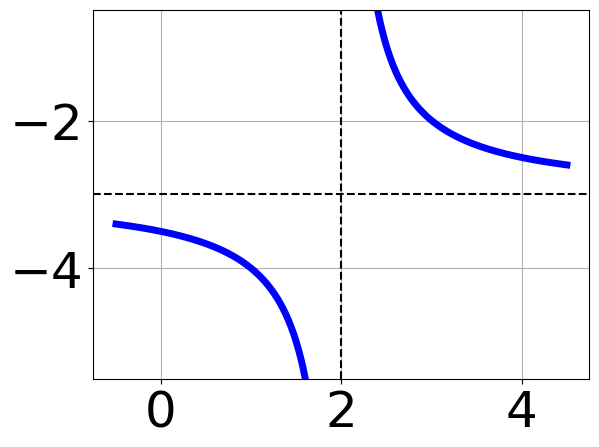
\includegraphics[width = 0.3\textwidth]{../Figures/rationalEquationToGraphCopyCC.png}\item 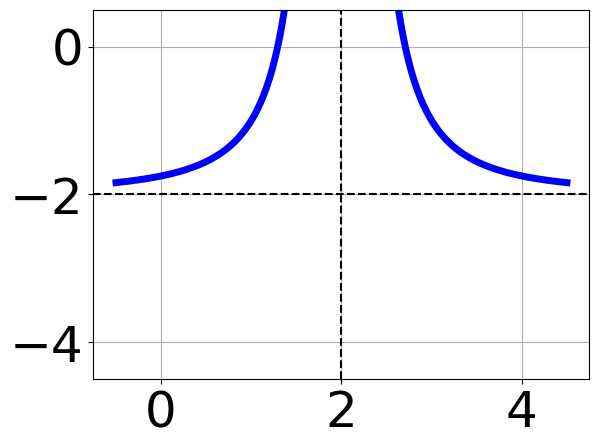
\includegraphics[width = 0.3\textwidth]{../Figures/rationalEquationToGraphCopyDC.png}\end{multicols}\item None of the above.
\end{enumerate} }
\end{enumerate}

\end{document}